\section{Parameters and Implementations}
\subsection{Parameters}
We use a same approach to derive the security of the parameters as in Squirrel \cite{CCS:FleSimZha22}.
We adopted the so-called ``realistic model'' in \cite{DBLP:conf/uss/AlkimDPS16}.
For a BKZ of block size $\beta$, the cost in this model is estimated by
$2^{0.292\beta+16.4+\log(\#\texttt{SVP calls})}$. 
In the meantime, the LWE-estimator \cite{DBLP:journals/jmc/AlbrechtPS15}
shows that for a root Hermite factor of $1.005$ we expect a block size of 286, which yields 112 bits security under the above model. 

We require the ring-SIS problem in \ref{lem:hvcprobhom} and \ref{lem:kots_correct} are hard. We ran a script that enumerates all possible 
parameters, in terms of the modulus of the rings, the arity of decomposition, etc., and finds the parameter sets that
allows for smallest signature size.

The following table summarize the results from the script.

% \begin{table}
% \input{scripts/chipmunk/params_table}
% \end{table}
\subsection{Comparisons}\label{ss:comparison}

We compare the performance of Chipmunk against both the trivial solution, i.e., repeating Falcon signature for $\rho$ times, and
Squirrel, the previous state of the ark. The data for Chipmunk and Squirrel are collected over a same platform: an AMD 5900x with 24 threads
and 32 Gigabytes of memory. The data for Falcon-512 is collected from their official website\footnote{\url{https://falcon-sign.info/}}.

The comparison with the trivial solution is quite straightforward. Since its signature size grows linearly with the number of signers,
Chipmunk can easily improve this by a couple of order of magnitudes.
In terms of Squirrel, we see that for both $\rho = 1024$ and $\rho = 8192$, our scheme is always better. 
In particular, there were two main obstacles that prevent Squirrel from being widely deployed, namely, the key generation time
and the signature size. We show that the key generation time is improved for 9 times over a same platform; and the 
aggregated signature is reduced by 5 times. 

\begin{table}\centering
  \begin{tabular}{|c||l|c|c|c||c|c|c|c||c|c|c|}\hline
    \# signers      &                 & Falcon$^{*}$& Squirrel$^{**}$  & Chipmunk$^{**}$  & Imp. Falcon & Imp. Squirrel \\\hline\hline
    \multirow{2}{*}{} 
                    & Key Generation  & 8.6 ms      & 4 min     & 26.5 sec  &     -       & 9.0$\times$ \\\cline{2-7}
                    & Signing         & 0.17 ms     & 2.1 ms    & 0.4 ms    &     -       & 5.2$\times$ \\\cline{2-7}
                    &Fresh Sig. Size  & 666 Bytes   & 45 KB     & 32 KB     &     -       & 1.4$\times$ \\\hline\hline
    \multirow{3}{*}{1024}                
                    &Aggregation      & -           & 1.2 sec   & 0.55 sec  &     -       & 2.2$\times$ \\\cline{2-7}
                    &Batch Verification    
                                      & 36.7 ms     & 19.5 ms   & 7.2 ms    & 5.1$\times$ & 2.7$\times$ \\\cline{2-7}
                    
                    &Agg. Sig. size   & 682 KB      & 572 KB    & 142 KB    & 4.8$\times$ & 4.0$\times$ \\\hline\hline
    \multirow{3}{*}{8192}                
                    &Aggregation      & -           & 9.6 sec   & 4.3 sec   &     -       & 2.2$\times$ \\\cline{2-7}
                    &Batch Verification    
                                      & 294 ms      & 53  ms    &  47 ms    & 6.2$\times$ & 1.1$\times$ \\\cline{2-7}
                    &Agg. Sig. size   & 5.5 MB      & 762 KB    & 160 KB    & 340$\times$ & 4.8$\times$ \\\hline
\end{tabular}\\
  $^{*}$: Trivial solution via repeating Falcon-512 signature for ``\# signers'' times.\\
  $^{**}$: Using parameters $\tau=21$.
  \caption{Comparisons among different solutions.}
\end{table}

\subsection{Practical performance}
To show that Chipmunk is practical, 
we take a deep dive into the two major obstacles, namely, the key generation time and the aggregated signature size.

We conduct a benchmark over a typical server that is equipped with AMD 7773x with
64 cores and 1 Terabytes of memory.
The results are summarized in Table \ref{tab:bench_results}.
Notice that this platform is different from that of Section \ref{ss:comparison}.

\begin{table}[t]\centering
  \begin{tabular}{|c|c||c||c|c|c|c|c|c||c|c|c|}\hline
      $\tau$              & Key Generation            & Signing                   & $\rho$  &  Aggregation & Verification  \\ \hline\hline
      \multirow{2}{*}{21} & \multirow{2}{*}{7.4 sec}  & \multirow{2}{*}{0.40 ms}  & 1024    &   491 ms     &  7.3 ms       \\\cline{4-6}
                          &                           &                           & 8192    &   3.5 sec    &  42.3 ms       \\\hline

      \multirow{2}{*}{24} & \multirow{2}{*}{59.8 sec} & \multirow{2}{*}{0.44 ms}  & 1024    &    ms     &   ms       \\\cline{4-6}
                          &                           &                           & 8192    &    sec    &   ms       \\\hline

      % \multirow{2}{*}{26} & \multirow{2}{*}{7.4 sec}  & \multirow{2}{*}{0.4 ms}   & 1024    &   491 ms     &  7.3 ms       \\\cline{4-6}
      %                     &                           &                           & 8192    &   3.5 sec    &  42.3 ms       \\\hline 

  \end{tabular}\\
  \caption{Benchmark results}
  \label{tab:bench_results}
\end{table}

% \end{table}
% \subsection{Micro Benchmarks}
We measure the time to generate the keys. As we shall see in Figure \ref{fig:keygen}, the key generation time scales linearly in the 
height of the tree. For the largest parameter set with $\tau = 26$, we can generate a keypair within 4 minutes, improving from 2 hours in Squirrel.
This is sufficient for 21 years of usage, assuming each block takes 10 seconds to finalize as in the case of Ethereum. 
We conclude that the key generation time is no longer a bottleneck for practical deployment.
\begin{figure}[H] 
  \centering
  \begin{subfigure}[b]
  {0.45\textwidth}    \centering
  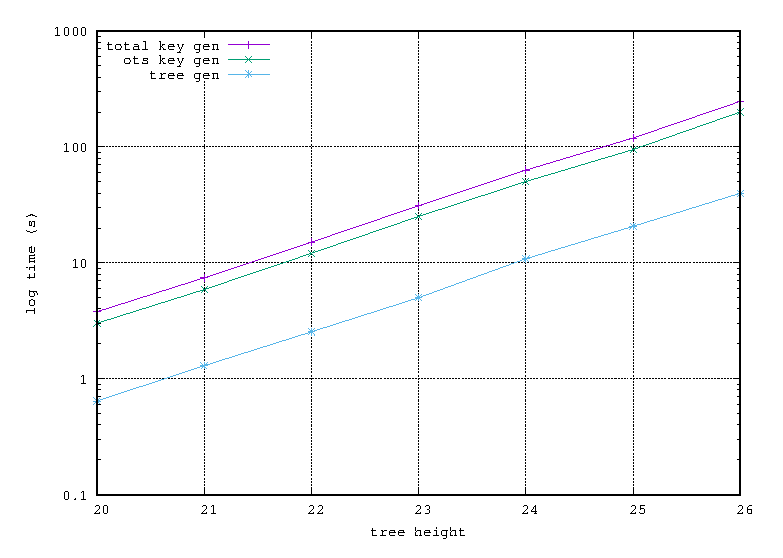
\includegraphics[width=\textwidth]{figures/key_gen.eps}\\
  \caption{Chipmunk key generations.}
  \label{fig:keygen}
  \end{subfigure}
~
\begin{subfigure}[b]{0.45\textwidth}    \centering
  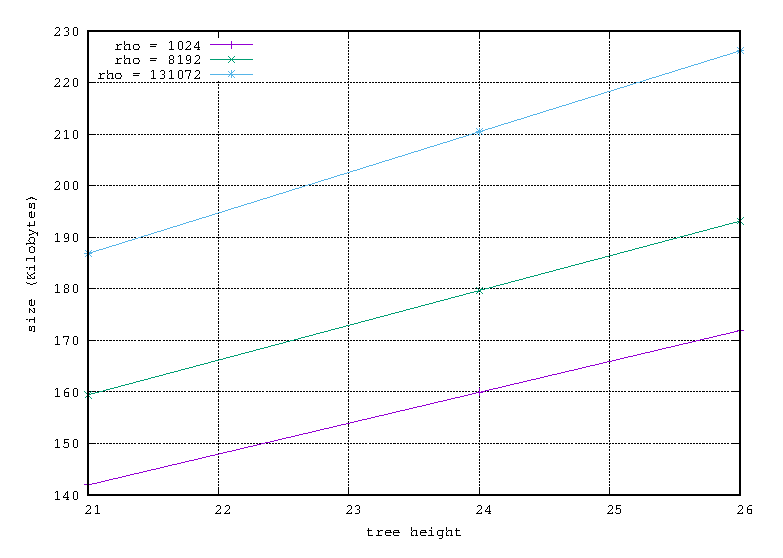
\includegraphics[width=\textwidth]{figures/sig_size.eps}\\
  \caption{Chipmunk aggregated signature size}
  \label{fig:sigize}
  \end{subfigure}

\end{figure}


% \subsection{Sizes}
In terms of the signature size, for the parameter set with $\tau=21$ and $\rho=1024$,
an aggregated signature is of size 142 Kilobytes, consists of 
\begin{itemize}
  \item the aggregated path to the root and its adjacent nodes, i.e., $2\tau\lceil\log(q, \eta)\rceil$ polynomials in $\mathcal{R}_q$ with an infinity norm bound $\beta <2^{15}$. This adds up to $126$ Kilobytes.
  \item the aggregated one time signature, i.e., $2\gamma$ polynomials in $\mathcal{R}_{q'}$ with norm bound $\beta_\sigma < 2^{20}$, or $16$ Kilobytes.
\end{itemize}
This merely fits inside an ethereum block whose peak size is around 130 Kilobytes to date\footnote{https://etherscan.io/chart/blocksize}.


